\documentclass[a4paper,11pt,fleqn,dvipsnames,twoside,openany]{memoir} 	% Openright aabner kapitler paa hoejresider (openany begge)

%%%% PACKAGES %%%%

% ¤¤ Oversaettelse og tegnsaetning ¤¤ %
\usepackage[utf8]{inputenc}					% Input-indkodning af tegnsaet (UTF8)
\usepackage[english]{babel}					% Dokumentets sprog
\usepackage[T1]{fontenc}					% Output-indkodning af tegnsaet (T1)
\usepackage{ragged2e,anyfontsize}			% Justering af elementer
\usepackage{fixltx2e}						% Retter forskellige fejl i LaTeX-kernen
																			
% ¤¤ Figurer og tabeller (floats) ¤¤ %
\usepackage{graphicx} 						% Haandtering af eksterne billeder (JPG, PNG, EPS, PDF)
%\usepackage{eso-pic}						% Tilfoej billedekommandoer paa hver side
%\usepackage{wrapfig}						% Indsaettelse af figurer omsvoebt af tekst. \begin{wrapfigure}{Placering}{Stoerrelse}
\usepackage{multirow}                		% Fletning af raekker og kolonner (\multicolumn og \multirow)
\usepackage{multicol}         	        	% Muliggoer output i spalter
\usepackage{rotating}						% Rotation af tekst med \begin{sideways}...\end{sideways}
\usepackage{colortbl} 						% Farver i tabeller (fx \columncolor og \rowcolor)
\usepackage[table]{xcolor}				 	% Definer farver med \definecolor. Se mere: http://en.wikibooks.org/wiki/LaTeX/Colors
\usepackage{flafter}						% Soerger for at floats ikke optraeder i teksten foer deres reference
\let\newfloat\relax 						% Justering mellem float-pakken og memoir
\usepackage{float}							% Muliggoer eksakt placering af floats, f.eks. \begin{figure}[H]


% ¤¤ Matematik mm. ¤¤
\usepackage{amsmath,amssymb,stmaryrd} 		% Avancerede matematik-udvidelser
\usepackage{mathtools}						% Andre matematik- og tegnudvidelser
\usepackage{textcomp}                 		% Symbol-udvidelser (f.eks. promille-tegn med \textperthousand )
\usepackage{rsphrase}						% Kemi-pakke til RS-saetninger, f.eks. \rsphrase{R1}
\usepackage[version=3]{mhchem} 				% Kemi-pakke til flot og let notation af formler, f.eks. \ce{Fe2O3}
\usepackage{siunitx}						% Flot og konsistent praesentation af tal og enheder med \si{enhed} og \SI{tal}{enhed}
\sisetup{locale=DE}							% Opsaetning af \SI (DE for komma som decimalseparator) 

% ¤¤ Referencer og kilder ¤¤ %
\usepackage[danish]{varioref}				% Muliggoer bl.a. krydshenvisninger med sidetal (\vref)
\usepackage{natbib}							% Udvidelse med naturvidenskabelige citationsmodeller
%\usepackage{xr}							% Referencer til eksternt dokument med \externaldocument{<NAVN>}
%\usepackage{glossaries}					% Terminologi- eller symbolliste (se mere i Daleifs Latex-bog)

% ¤¤ Misc. ¤¤ %
\usepackage{lipsum}							% Dummy text \lipsum[..]
\usepackage[shortlabels]{enumitem}			% Muliggoer enkelt konfiguration af lister
\usepackage{pdfpages}						% Goer det muligt at inkludere pdf-dokumenter med kommandoen \includepdf[pages={x-y}]{fil.pdf}	
\pdfoptionpdfminorversion=6					% Muliggoer inkludering af pdf dokumenter, af version 1.6 og hoejere
\pretolerance=2500 							% Justering af afstand mellem ord (hoejt tal, mindre orddeling og mere luft mellem ord)

% Kommentarer og rettelser med \fxnote. Med 'final' i stedet for 'draft' udloeser hver note en error i den faerdige rapport.
\usepackage[footnote,draft,danish,silent,nomargin]{fixme}		
\usepackage[bottom]{footmisc}

%%%% CUSTOM SETTINGS %%%%

% ¤¤ Marginer ¤¤ %
\setlrmarginsandblock{3.5cm}{2.5cm}{*}		% \setlrmarginsandblock{Indbinding}{Kant}{Ratio}
\setulmarginsandblock{2.5cm}{3.0cm}{*}		% \setulmarginsandblock{Top}{Bund}{Ratio}
\checkandfixthelayout 						% Oversaetter vaerdier til brug for andre pakker

%	¤¤ Afsnitsformatering ¤¤ %
\setlength{\parindent}{0mm}           		% Stoerrelse af indryk
\setlength{\parskip}{3mm}          			% Afstand mellem afsnit ved brug af double Enter
\linespread{1,1}							% Linie afstand

% ¤¤ Litteraturlisten ¤¤ %
\bibpunct[,]{[}{]}{;}{a}{,}{,} 				% Definerer de 6 parametre ved Harvard henvisning (bl.a. parantestype og seperatortegn)
\bibliographystyle{bibtex/harvard}			% Udseende af litteraturlisten.

% ¤¤ Indholdsfortegnelse ¤¤ %
\setsecnumdepth{subsection}		 			% Dybden af nummerede overkrifter (part/chapter/section/subsection)
\maxsecnumdepth{subsection}					% Dokumentklassens graense for nummereringsdybde
\settocdepth{subsection} 					% Dybden af indholdsfortegnelsen

% ¤¤ Lister ¤¤ %
\setlist{
  topsep=0pt,								% Vertikal afstand mellem tekst og listen
  itemsep=-1ex,								% Vertikal afstand mellem items
} 

% ¤¤ Visuelle referencer ¤¤ %
\usepackage[colorlinks]{hyperref}			% Danner klikbare referencer (hyperlinks) i dokumentet.
\hypersetup{colorlinks = true,				% Opsaetning af farvede hyperlinks (interne links, citeringer og URL)
    linkcolor = black,
    citecolor = black,
    urlcolor = black
}

% ¤¤ Opsaetning af figur- og tabeltekst ¤¤ %
\captionnamefont{\small\bfseries\itshape}	% Opsaetning af tekstdelen ('Figur' eller 'Tabel')
\captiontitlefont{\small}					% Opsaetning af nummerering
\captiondelim{. }							% Seperator mellem nummerering og figurtekst
\hangcaption								% Venstrejusterer flere-liniers figurtekst under hinanden
\captionwidth{\linewidth}					% Bredden af figurteksten
\setlength{\belowcaptionskip}{10pt}			% Afstand under figurteksten
		
% ¤¤ Navngivning ¤¤ %
\addto\captionsdanish{
	\renewcommand\appendixname{Appendiks}
	\renewcommand\contentsname{Indholdsfortegnelse}	
	\renewcommand\appendixpagename{Appendiks}
	\renewcommand\appendixtocname{Appendiks}
	\renewcommand\cftchaptername{\chaptername~}				% Skriver "Kapitel" foran kapitlerne i indholdsfortegnelsen
	\renewcommand\cftappendixname{\appendixname~}			% Skriver "Appendiks" foran appendiks i indholdsfortegnelsen
}

% ¤¤ Kapiteludssende ¤¤ %
\definecolor{numbercolor}{gray}{0.7}		% Definerer en farve til brug til kapiteludseende
\newif\ifchapternonum

\makechapterstyle{E4}{					% Definerer kapiteludseende frem til ...
  \renewcommand\beforechapskip{0pt}
  \renewcommand\printchaptername{}
  \renewcommand\printchapternum{}
  \renewcommand\printchapternonum{\chapternonumtrue}
  \renewcommand\chaptitlefont{\fontfamily{pbk}\fontseries{db}\fontshape{n}\fontsize{25}{35}\selectfont\raggedleft}
  \renewcommand\chapnumfont{\fontfamily{pbk}\fontseries{m}\fontshape{n}\fontsize{1in}{0in}\selectfont\color{numbercolor}}
  \renewcommand\printchaptertitle[1]{%
    \noindent
    \ifchapternonum
    \begin{tabularx}{\textwidth}{X}
    {\let\\\newline\chaptitlefont ##1\par} 
    \end{tabularx}
    \par\vskip-2.5mm\hrule
    \else
    \begin{tabularx}{\textwidth}{Xl}
    {\parbox[b]{\linewidth}{\chaptitlefont ##1}} & \raisebox{-15pt}{\chapnumfont \thechapter}
    \end{tabularx}
    \par\vskip2mm\hrule
    \fi
  }
}											% ... her

\chapterstyle{E4}						% Valg af kapiteludseende - Google 'memoir chapter styles' for alternativer

% ¤¤ Sidehoved ¤¤ %

\makepagestyle{IHA}							% Definerer sidehoved og sidefod udseende frem til ...
\makepsmarks{IHA}{%
	\createmark{chapter}{left}{shownumber}{}{. \ }
	\createmark{section}{right}{shownumber}{}{. \ }
	\createplainmark{toc}{both}{\contentsname}
	\createplainmark{lof}{both}{\listfigurename}
	\createplainmark{lot}{both}{\listtablename}
	\createplainmark{bib}{both}{\bibname}
	\createplainmark{index}{both}{\indexname}
	\createplainmark{glossary}{both}{\glossaryname}
}
\nouppercaseheads											% Ingen Caps oenskes

\makeevenhead{IHA}{}{}{\leftmark}				% Definerer lige siders sidehoved (\makeevenhead{Navn}{Venstre}{Center}{Hoejre})
\makeoddhead{IHA}{\rightmark}{}{Ingeniørhøjskolen i Aarhus}		% Definerer ulige siders sidehoved (\makeoddhead{Navn}{Venstre}{Center}{Hoejre})
\makeevenfoot{IHA}{\thepage}{}{}							% Definerer lige siders sidefod (\makeevenfoot{Navn}{Venstre}{Center}{Hoejre})
\makeoddfoot{IHA}{}{}{\thepage}								% Definerer ulige siders sidefod (\makeoddfoot{Navn}{Venstre}{Center}{Hoejre})
\makeheadrule{IHA}{\textwidth}{0.5pt}						% Tilfoejer en streg under sidehovedets indhold
\makefootrule{IHA}{\textwidth}{0.5pt}{1mm}					% Tilfoejer en streg under sidefodens indhold

\copypagestyle{IHAchap}{IHA}								% Sidehoved for kapitelsider defineres som standardsider, men med blank sidehoved
\makeoddhead{IHAchap}{}{}{}
\makeevenhead{IHAchap}{}{}{}
\makeheadrule{IHAchap}{\textwidth}{0pt}
\aliaspagestyle{chapter}{IHAchap}							% Den ny style vaelges til at gaelde for chapters
															% ... her
															
\pagestyle{IHA}												% Valg af sidehoved og sidefod


%%%% CUSTOM COMMANDS %%%%

% ¤¤ Billede hack ¤¤ %
\newcommand{\figur}[4]{
		\begin{figure}[H] \centering
			\includegraphics[width=#1\textwidth]{billeder/#2}
			\caption{#3}\label{#4}
		\end{figure} 
}

% ¤¤ Specielle tegn ¤¤ %
\newcommand{\grader}{^{\circ}\text{C}}
\newcommand{\gr}{^{\circ}}
\newcommand{\g}{\cdot}


%%%% ORDDELING %%%%

\hyphenation{}

%%%% FARVER %%%%
\definecolor{light-gray}{gray}{0.95}
\raggedbottom
\begin{document}

\pagestyle{empty}
\newcommand{\HRule}{\rule{\linewidth}{0.5mm}} % Defines a new command for the horizontal lines, change thickness here

\begin{center} % Center everything on the page
 
%----------------------------------------------------------------------------------------
%	HEADING SECTIONS
%----------------------------------------------------------------------------------------

\textsc{\LARGE Ingeniørhøjskolen Århus}\\[1.5cm] % Name of your university/college
\textsc{\large Efterår 2013}\\[0.5cm] % Minor heading such as course title

%----------------------------------------------------------------------------------------
%	TITLE SECTION
%----------------------------------------------------------------------------------------

\HRule \\[0.4cm]
{ \huge \bfseries Forprojekt til bachelor}\\[0.4cm] % Title of your document
\HRule \\[1.5cm]
 
%----------------------------------------------------------------------------------------
%	AUTHOR SECTION
%----------------------------------------------------------------------------------------

\begin{table}[H]
    \begin{tabular}{|l|l|l|p{4cm}|}
    \hline
    Projekttitel: & \multicolumn{3}{|c|}{Charcot-Fod - Design og udvikling af temperatur-måle-device}                               \\ \hline
    Projektnr.   & Udbyder                                                     & Vejleder                & Bivejleder                     \\ \hline
    14030        & Delta                                                       & PKI@iha.dk              & ~                              \\ \hline
    Deltager 1:  & Studienr: 10734                                             & Navn: Johnny Kristensen & Underskrift: \_\_\_\_\_\_\_\_\_\_\_\_\_\_ \\ \hline
    Deltager 2:  & Studienr: 20093625                                          & Navn: Nicolai Glud      & Underskrift: \_\_\_\_\_\_\_\_\_\_\_\_\_\_ \\ \hline
    \end{tabular}

\end{table}

\ \\
\ \\
\ \\
\ \\
\ \\
\ \\
\begin{table}[H]
\begin{tabular}{|p{8.77cm}|c|c|}
	\hline
	\multicolumn{3}{|c|}{\huge Evaluering af Forprojektet}\\
	\multicolumn{3}{|c|}{Vejleder afleverer kopi af denne side \textbf{SENEST 24. januar 2014}, til studiekontoret!}\\ \hline
    Evaluaringsdato: & Sæt kryds & Sæt kryds\\
    ~&  ~ & ~\\ \cline{1-1} 
    Vejleders underskrift & Godkendt & IKKE Godkendt \\
    ~ & ~ & ~  \\\hline
    \end{tabular}
\end{table}
%----------------------------------------------------------------------------------------

\vfill % Fill the rest of the page with whitespace
%----------------------------------------------------------------------------------------
%	DATE SECTION
%----------------------------------------------------------------------------------------

{\large \today}\\[3cm] % Date, change the \today to a set date if you want to be precise
\end{center}

\pagestyle{plain}

% Opgavebeskrivelsen fra projektkataloget
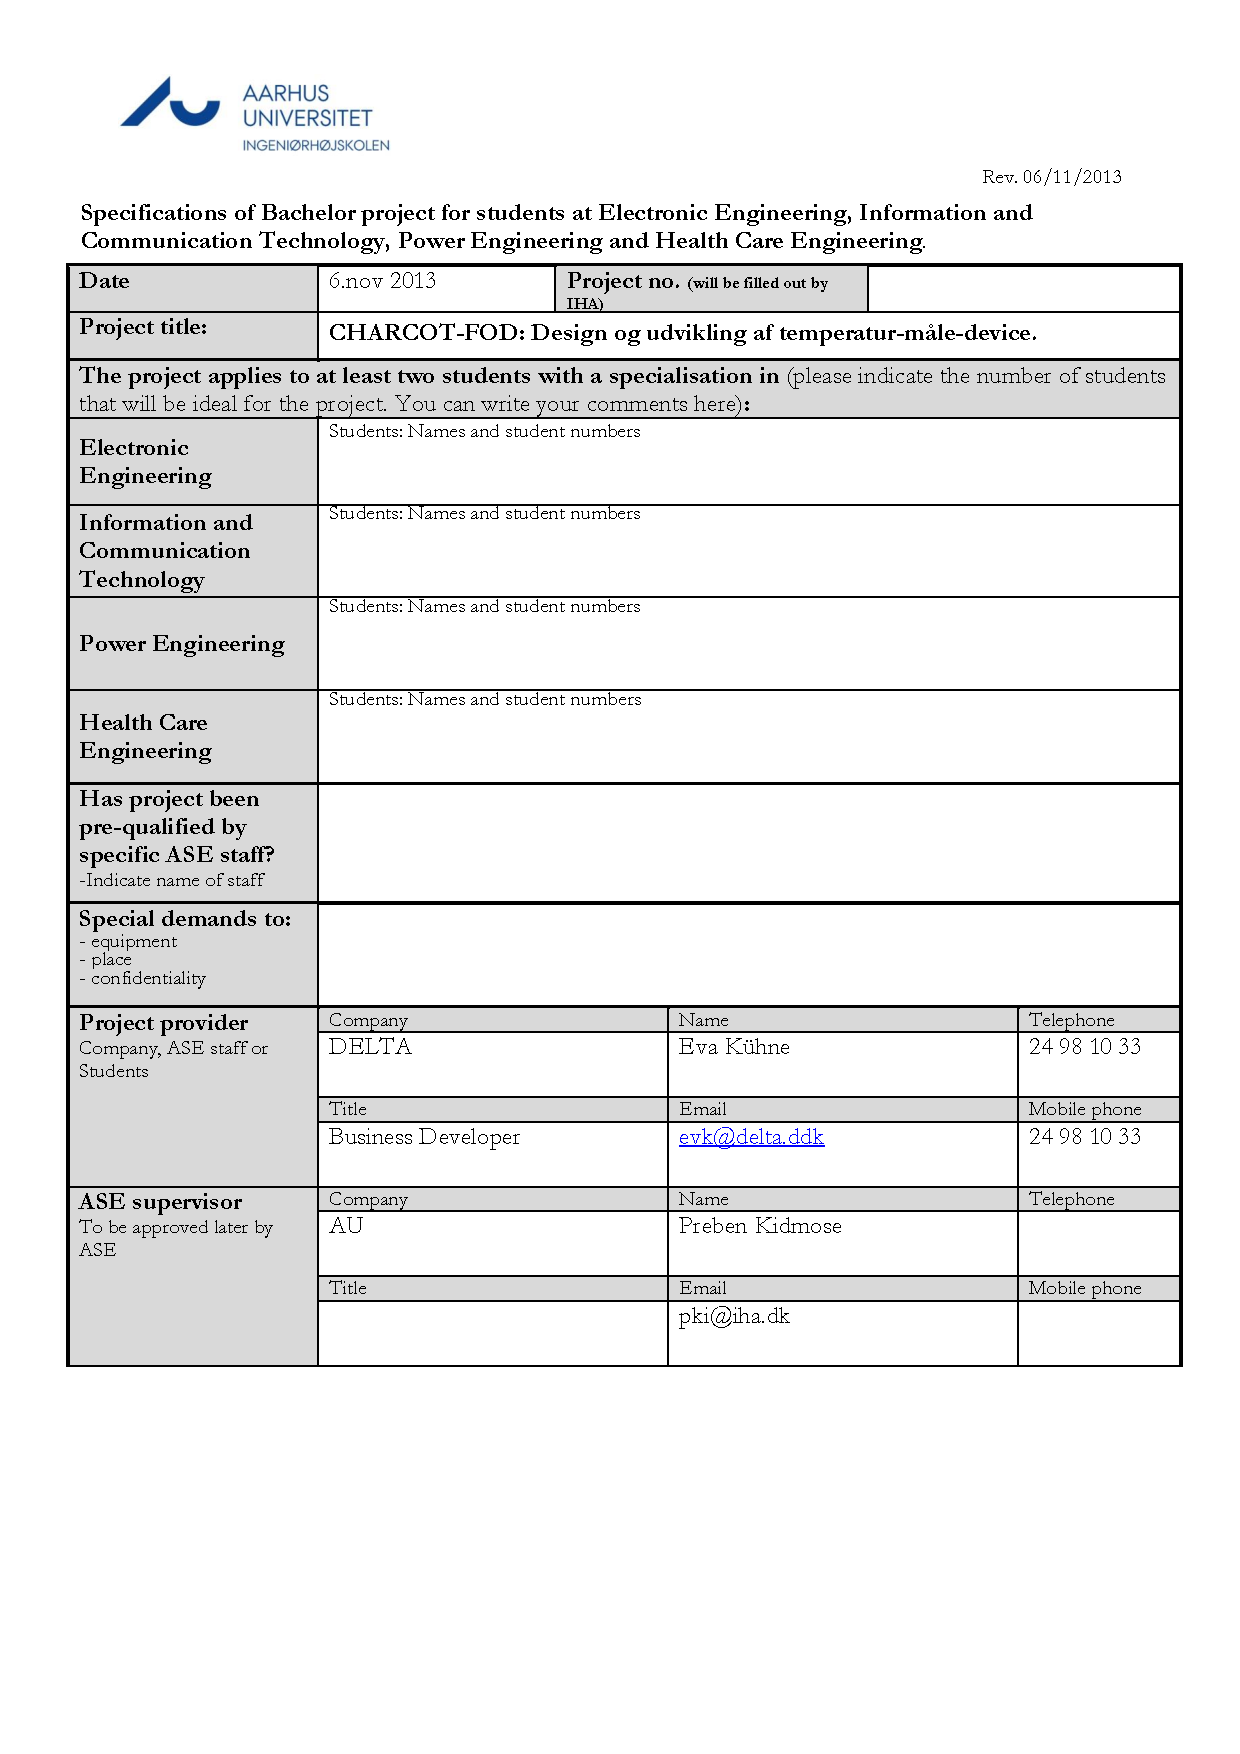
\includepdf[pages=-]{filer/opgavebeskrivelse.pdf}

% Udkast til projektbeskrivelse
\chapter{Project description - extension}
This project description is an extension of the original project description made by Delta. It is made to clarify the borders and content of the bachelor project at the engineering college of Aarhus.\\
The description discards irrelevant subjects or elements of no interest. It adds new elements relevant for the students which is still in the range of the original project description.\\
The name of the project will be "Charcot foot prevention system".


\section{Background}
The original project description did not fulfil the demands to a bachelor project with regards to new technology and new knowledge. Therefore the original project description needs to be modified to accommodate the group and the supervisors requirements to a bachelors project. \\
This twist of the project has been made in collaboration with the project supervisor.\\
The extension includes new communication protocol development and smart-sensor development.\\
Therefore this project will lead more towards a conceptual development project than a real development project.\\


\section{Project description}
The new focus will be upon the temperature and accelerometer sensors and the development of a system with one or max two wires connecting the sensors. The sensors will be interconnected and connected to the Central data unit. Temperature sensors will be addressed by the Central data  unit. Data will be stored by the Central data unit for possible extraction by a user interface. \\

The main idea behind the temperature and accelerometer sensors points toward a prototype PCB with discrete components. The sensor board prototype board will be made on a large PCB with a simple layout to prove that the concept is possible. \\

For development purposes a grid line will be used to power the Central data unit. A development kit or board for the microprocessor or controller  will be used while developing the brain of the central data unit. \\

\section{Final Product}
\textit{The final product is out of our scope. For full understanding of the system the final product description is included in this section.}\\

The final product will entail a computer and a smart-phone to read data from the central data unit. They will also carry the alarms and messages from the system to the user. Further more it is possible to check the data history on these units. \\

The prototype sensor board is supposed to be made into an embedded IC which will be sealed with epoxy to fulfil the demand for hygiene and cleaning. The size of the embedded IC will also be small enough so that is does not interfere with the daily life of the user. The sensor IC will be placed in a sock for the user to wear. \\

The Central data collection unit will run on a rechargeable battery. This will allow the user to recharge the system over night and then use it during the day without being confined by grid wires.\\

Data can be extracted from the central data unit with a wireless protocol, a replaceable data card or with a USB protocol.
\begin{figure}[H]
\centering
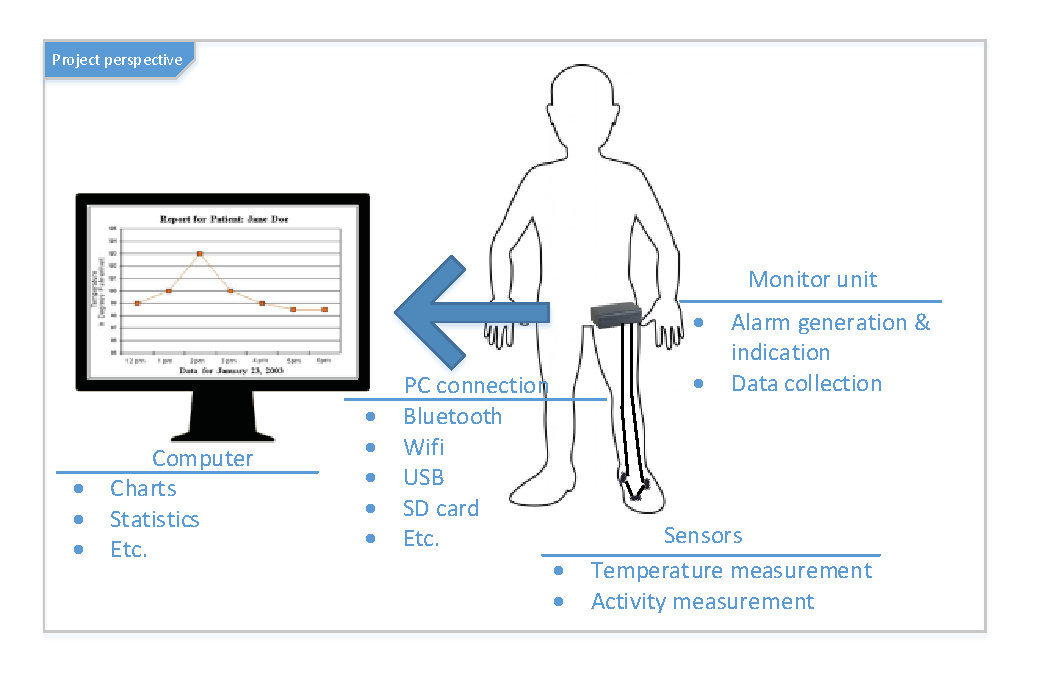
\includegraphics[width=0.8\textwidth]{billeder/fullsystem_vector}
\caption{The full system in perspective to the project.}
\end{figure}
 

% Udkast til kravspecifikation
%A good requirement is:
%*Correct
%*Unambiguous (all statements have exactly one interpretation)
%*Complete (where TBDs are absolutely necessary, document why the information is unknown, who is responsible for resolution, and the deadline)
%*Consistent
%*Ranked for importance and/or stability
%*Verifiable (avoid soft descriptions like “works well”, “is #user frndly”; use concrete terms and specify measurable #quantities)
%*Modifiable (evolve the Requirements Specification only via a #formal change process, preserving a complete audit trail of #changes)
%*Does not specify any particular design
%*Traceable (cross-reference with source documents and spawned documents).




\chapter{Requirement specification}

\section{Version history}
\begin{table}[H]
\begin{tabular}{|c|p{9cm}|c|c|}
\hline
Version & Description & Author & Date\\
\hline
0.1 & Initial draft & JK & 21/12-13\\
\hline
\end{tabular}
\end{table}

\section{Purpose}
The purpose of this document is to present a detailed description of the Charcot foot prevention system. It thoroughly outlines and specifies the features, interfaces, purpose of the system as well as under which constraints the system will operate under.\\
The intended audience of the document is the developers, the supervisor and Delta.\\
The requirements of the system may only be changed after a review meeting with the group and stakeholders.\\

\section{Scope of project}


\section{References}
Project description

\section{Glossary}
\begin{table}[H]
\centering
\begin{tabular}{|p{4cm}|p{7cm}|}
\hline
Term & Definition\\ \hline
CDU & Abbreviation of "Central Data Unit", a key component in the system. \\ \hline
Delta & The company which this project is made in collaboration with.\\ \hline
BOM & Build Of Material abbreviation\\ \hline
\end{tabular}
\end{table}

\section{General description}

\subsection{General System}
\begin{figure}[H]
	\centering
	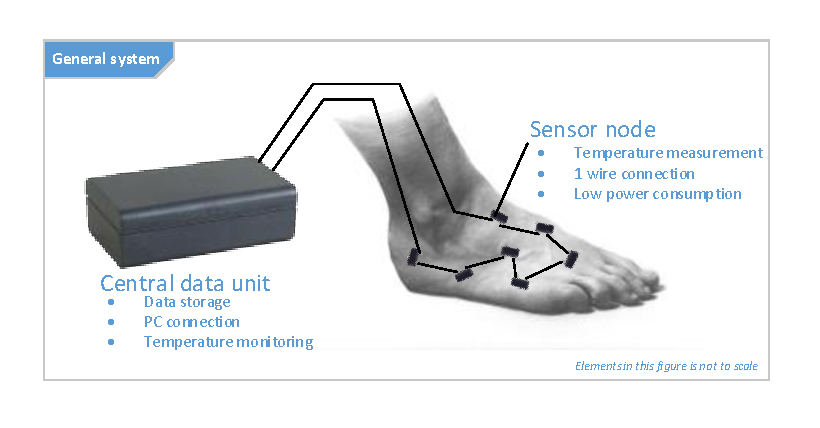
\includegraphics[width=0.8\textwidth]{billeder/GeneralSystem}
	\caption{General System}
\end{figure}

\subsection{System description}
Et device der skal påmonteres foden på en person der er disponeret til at udvikle Charcotfod. Devicet skal ud fra temperatur og aktivitetsniveau finde ud af om der er en fare for overbelastning. Hvis dette er tilfældet skal brugeren advares.

\subsection{Constraints}
\textit{Currently none.}
\subsection{Dependencies}
\textit{Currently none.}

%\subsection{Prototype af UI eller GUI}

%\subsection{Beskrivelse af UI eller GUI}

\section{Functional requirements}
Below is listed all functional requirements to the system.\\
\textbf{\large{Priority definitions}}\\
The following definitions are intended as a guideline to prioritize requirements.
\begin{itemize}[noitemsep,nolistsep]
\item Priority 1 - This is a "Need to Have" either defined by law or of most importance of the project.
\item Priority 2 - This requirement is if high importance and will be of great benefit for the system
\item Priority 3 - This requirement will be great to have but not important
\item Priority 4 - This requirement is purely "Nice-to-have" and will not be considered unless there is time to spare.
\end{itemize}


\subsection{Actors of the system}

\subsubsection{Primary actors}

\begin{table}[H]
	\centering
	\begin{tabular}{|l|p{7cm}|}
	\hline
	Actor name & Central data unit \\ \hline
	Type & Primary \\ \hline
	Description & The Central data unit is the main actor of the system. The Central data unit contacts sensors and manage data. It consists of a microcontroller and some memory for data. \\ \hline
	\end{tabular}
\end{table}

\begin{table}[H]
	\centering
	\begin{tabular}{|l|p{7cm}|}
	\hline
	Actor name & Patient \\ \hline
	Type & Primary \\ \hline
	Description &  The patient set the system to run and initiates data extraction from the CDU.\\ \hline
	\end{tabular}
\end{table}

\subsubsection{Secondary actors}

\begin{table}[H]
	\centering
	\begin{tabular}{|l|p{7cm}|}
	\hline
	Actor name & Sensor \\ \hline
	Type & Secondary \\ \hline
	Description & The sensor actor consists of a sensor, a microcontroller and a powercontrol unit. It responds to messages initiated by the central data unit.\\ \hline
	\end{tabular}
\end{table}

\begin{table}[H]
	\centering
	\begin{tabular}{|l|p{7cm}|}
	\hline
	Actor name & Computer \\ \hline
	Type & Secondary \\ \hline
	Description & The computer can extract data from the central data unit. It is not intended as a control unit but mostly just for demonstration purposes. \\ \hline
	\end{tabular}
\end{table}




\subsection{Use Case diagram}
Below is shown the use case diagram.
\begin{figure}[H]
\centering
\includegraphics[width=.8\textwidth]{billeder/usecase_fig.png}
\label{usecase_fig}
\caption{Use case diagram}
\end{figure}

\subsection{Use Cases}

\subsubsection{Set system to normal operation}

\begin{table}[H]
	\centering
	\begin{tabular}{|l|p{10cm}|}
	\hline
	Goal 							& To set the system to normal operatio.n \\ \hline
	Initialisation 					& The Patient initiates the use case. \\ \hline
	\multirow{2}{*}{Actors} 		& Patient \\ 
									& CDU \\ \hline
	Reference 						& Get data from sensor \#X \\ \hline
	\# of concurrent events 		& 1 \\ \hline
	Prerequisite  					& The patient connect the sensors to the port on the CDU. \\ \hline
	Post condition 					& The system is set to normal operation. \\ \hline
	\multirow{5}{*}{Main Scenario} 	& 1. The patient clicks the  "ON"-button. \\
	& 2. The CDU checks if the sensors are connected.\\
	& 3. The CDU scans for sensors within address range and stores the addresses along with a sensor numbers.\\ 
	& 4. The CDU checks if the memory is responding.\\
	& 5. The CDU reads which memory space is being used from the memory.\\ \hline
	\multirow{6}{*}{Exceptions} & 2a. The sensors are not connected \\ 
								& - The CDU indicates an error and stops operation.\\											& 2b. There is no response from any sensor\\
								& - The CDU indicates an error and stops operation. \\
								& 4c. The memory is not responding\\
								& - The CDU indicates an error and stops operation. \\ 
								\hline
	Priority					& 1\\\hline
	\end{tabular}
\end{table}

\subsubsection{Get data from sensor \#X}
\begin{table}[H]
	\centering
	\begin{tabular}{|l|p{10cm}|}
	\hline
	Goal 							& Collect data from a sensor. \\ \hline
	Initialisation 					& The CDU runs a cycle and each cycle collects data from each sensor. The CDU then initiates the get data from sensor when it is time. \\ \hline
	\multirow{2}{*}{Actors} 		& CDU \\ 
									& Sensor \\ \hline
	\multirow{2}{*}{Reference}		& Set system to normal operation \\ 
									& Store data \\\hline
	\# of concurrent events 		& 1 \\ \hline
	Prerequisite  					& The usecase "Set system to normal operation" must have been completed. \\ \hline
	Post condition 					& Data has been acquired from sensor \#X \\ \hline
	\multirow{5}{*}{Main Scenario} 	& 1. The CDU determines which sensor to collect data from. \\
	& 2. The CDU contacts the sensor with the correct address and a command to send data back.\\
	& 3. The sensor responds with the data.\\ 
	& 4. The CDU validates if the data is within reasonable range. \\
	& 5. Initiates use case "Store data".\\ \hline
	\multirow{8}{*}{Exceptions} & 2a. The CDU cannot send data \\ 
								& - The CDU indicates an error and stops operation.\\											& 3b. There is no response from sensor\\
								& - The CDU indicates an error and continues operation. \\
								& 4c. The data is out of reasonable range.\\
								& - The CDU reinitiates the use case "Collect data from a sensor". \\ 
								& 4d. The data is out of reasonable range 3 times in a row with the same sensor. \\
								& - The CDU indicates an error and continues operation.\\ \hline
	Priority					& 1\\\hline
	\end{tabular}
\end{table}

\subsubsection{Store data}
\begin{table}[H]
	\centering
	\begin{tabular}{|l|p{10cm}|}
	\hline
	Goal 							& Save the data on memory \\ \hline
	Initialisation 					& The CDU initiates this use case once "Get data from \#X" has been completed. \\ \hline
	\multirow{1}{*}{Actors} 		& CDU \\ \hline
	Reference 						& Get data from sensor \#X. \\ \hline
	\# of concurrent events 		& 1 \\ \hline
	Prerequisite  					& The use case "Get data from sensor \#X" must have been completed. \\ \hline
	Post condition 					& Data has been stored on memory \\ \hline
	\multirow{4}{*}{Main Scenario} 	& 1. The CDU initiates the save data sequence because new data has been acquired from a sensor. \\
									& 2. The CDU gives the data a timestamp and the correct sensor number.\\
									& 3. The CDU transfers the data to the memory.\\ 
									& 4. The CDU reads the data again from the memory to ensure the data has been stored correctly. \\ \hline
	\multirow{4}{*}{Exceptions} & 3a. The CDU cannot transfer data. \\ 
								& - The CDU indicates an error and stops operation.\\											& 4a. The data was not stored correctly. \\
								& - The CDU reinitiates the "Store data" use case.\\\hline
	Priority					& 1\\\hline
	\end{tabular}
\end{table}

\subsubsection{Extract data from CDU}
\begin{table}[H]
	\centering
	\begin{tabular}{|l|p{10cm}|}
	\hline
	Goal 							& Extract the data from CDU.\\ \hline
	Initialisation 					& The patient connects the CDU to a computer. \\ \hline
	\multirow{3}{*}{Actors} 		& Patient \\ 
									& CDU \\
									& Computer \\\hline
	Reference 						& None \\ \hline
	\# of concurrent events 		& 1 \\ \hline
	Prerequisite  					& The system has been collecting data.\\ \hline
	Post condition 					& The data has been transferred to a computer. \\ \hline
	\multirow{4}{*}{Main Scenario} 	& 1. The patient disconnects the CDU from the sensors and connects it to the computer. \\
									& 2. The patient opens the program to transfer data.\\
									& 3. The patient sets up the program and sends the transfer command.\\ 
									& 4. The CDU responds with the data. \\ \hline
	\multirow{4}{*}{Exceptions} & 4a. The CDU does not respond. \\ 
								& - The CDU and computer are not connected correctly.\\											& 4b. The CDU responds "There is no data". \\
								& - There is not data on the CDU to respond with.\\\hline
	Priority					& 3\\\hline
	\end{tabular}
\end{table}

\section{Non functional requirements}
Below is listed all non-functional requirements. \\

\subsection{General requrements}
\begin{table}[H]
\begin{tabular}{p{10cm} p{2cm}}
$\bullet$ The system should be simple and not be of any discomfort of the patient. & \\
$\bullet$ The system should be small enough to have on a belt or similar and in a sock or shoe. &\\
$\bullet$ BOM Price & 40€\\
\end{tabular}
\end{table}


\subsection{Temperature sensor requirements}

\subsubsection{Functionality Requirements}
\begin{table}[H]
\begin{tabular}{p{10cm} p{2cm}}
$\bullet$ Accuracy: & <$0.5^o$C\\
$\bullet$ Update rate: & 5 sec\\
$\bullet$ Lifespan: & > 3 year\\
\end{tabular}
\end{table}

\subsubsection{Hardware Requirements}
%Krav til hardware (if any)\\
\begin{table}[H]
\begin{tabular}{p{10cm} p{2cm}}
$\bullet$ Power consumption: & <0.1W\\


\end{tabular}
\end{table}


\subsubsection{Software Requirements}
%Krav til software (if any)\\
\begin{table}[H]
\begin{tabular}{p{10cm} p{2cm}}
$\bullet$ Timer & Yes\\


\end{tabular}
\end{table}


\subsubsection{External interfaces}
\begin{table}[H]
\begin{tabular}{p{10cm} p{2cm}}
$\bullet$ 1 wire protocol & Yes\\
$\bullet$ Wires in: & 1\\
$\bullet$ Wires out: & 1\\
\end{tabular}
\end{table}

\subsection{Central data unit requirements}

\subsubsection{Functionality Requirements}
\begin{table}[H]
\begin{tabular}{p{10cm} p{2cm}}
$\bullet$ Cycle\footnotemark & 1 min\\
\end{tabular}
\end{table}
\footnotetext{In a cycle the CDU will collect data once from all sensors}
\subsubsection{Hardware Requirements}
%Krav til hardware (if any)\\
\begin{table}[H]
\begin{tabular}{p{10cm} p{2cm}}
$\bullet$ Power consumption: & <0.5W \footnotemark \\
$\bullet$ Memory: & >1MB\footnotemark\\
$\bullet$ Real time clock & Yes\\
\end{tabular}
\end{table}
\footnotetext{Sensor supply excluded}
\footnotetext{Or at least enough to store data for an entire day}

\subsubsection{Software Requirements}
%Krav til software (if any)\\
\begin{table}[H]
\begin{tabular}{p{10cm} p{2cm}}
$\bullet$ Save entries must contain: &Sensor nr. \\
~ 									&Temperatur. \\
~									&Timestamp. \\


\end{tabular}
\end{table}


\subsubsection{External interfaces}
\begin{table}[H]
\begin{tabular}{p{10cm} p{2cm}}
$\bullet$ 1 wire protocol & Yes\\
$\bullet$ CDU to computer interface & Yes\\
\end{tabular}
\end{table}

\subsection{Project requirements}

\subsubsection{Documentation}
\begin{itemize}
\item Engelsk
\item SysML
\end{itemize}

\subsubsection{Technologies and tools}
\begin{itemize}
\item Matlab
\item Maple/Mathcad
\item Microsoft Visio 2010/2013
\item TortoiseSVN
\item TeXmaker
\end{itemize}

\subsubsection{Misc}
\begin{itemize}
\item Report is written in LaTeX.
\end{itemize}

\section{List of figures}

% Udkast til projektplan, herunder beskrivelser af hvilke eksperimenter, teknologier mm der forventes udarbejdet i løbet af afgangsprojektet
\chapter{Project planning}
\section{Time schedule}
Below is shown the preliminary time schedule of the project. This schedule will change and must be versionized with every change and updated with regards to time on tasks, tasks and details.\\ 

\begin{table}[H]
\centering
\begin{tabular}{|l |p{4cm} |c |c |c |c |c|}
\hline 
$\#$ & Task Name & Duration(d) & Start & Finish & Predecessor & Resources \\ 
\hline 
1 & System design & 10 days & 03-feb & 14-feb & none & NG \& JK \\ 
\hline
1-1 & Acceptance test & * & * & * & none &  NG \& JK \\ 
\hline
2 & Technology dev and research & 10 days & 17-feb & 28-feb & $\#$1 & NG \& JK \\ 
\hline 
3 & Development phase & 43 days & 03-mar & 30-apr & $\#$2 & NG \& JK \\ 
\hline 
5 & Finalize documentation & 7 days & 01-may & 9-may & $\#$1,2,3,4 & NG \& JK \\ 
\hline 
6 & Report & 20 days & 5-may & 30-jun & $\#$1,2,3,4,(5) & NG \& JK \\ 
\hline \hline
~ & In total & 85 days & 03-feb & 30-may & ~ & ~ \\ 
\hline 
\end{tabular} 
\end{table}

\begin{figure}[H]
\centering
\includegraphics[width=.9\textwidth]{billeder/timeschedule_vector}
\caption{Time schedule}
\end{figure}

\section{Experiments}
\subsection{Determine the optimal placement for sensors}
A possible extension of the project will be to apply the sensors to a foot and check whether the system works as intended. In this regard the optimal sensor placement will be preferable to determine.\\
This could be determined by examining heat maps of charcot feet.\\
This experiment is at the moment not intended as a part of this project.

\subsection{Field test of sensor unit}
It will be most natural to apply a sensor unit to a foot to determine the temperature of the foot. This way we will be able to determine if the sensor need to be applied directly to the skin or if they work by close proximity. 

\section{Project organizing}
This section describes organizing, planning and other practical aspects of the project.

\subsection{Project flow}
The project work shall follow an iterative process were each phase will be repeated several times. The amount of work put into each task can vary from time to time and will be decided by the group members each time depending on how much is needed. Below is shown a figure describing the project flow. If the method and work flow doesn't work as intended the procedure can be altered at all times during the project.
\begin{figure}[H]
\centering
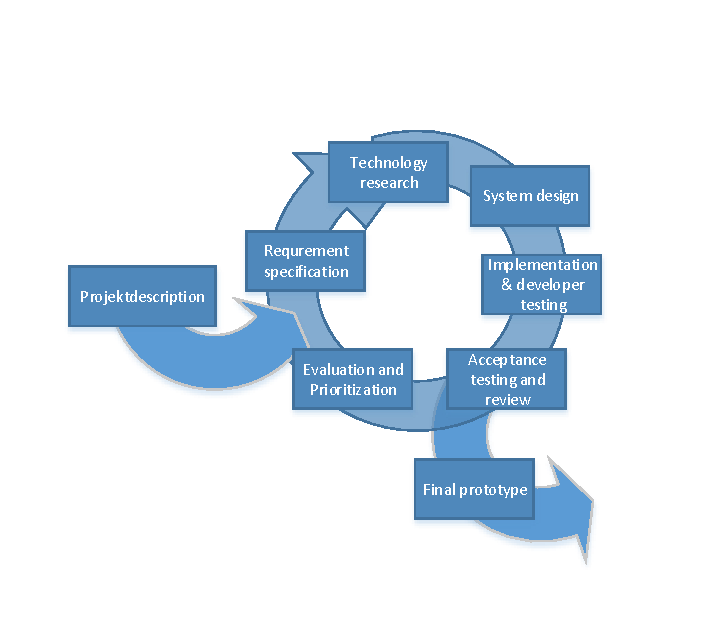
\includegraphics[width=.8\textwidth]{billeder/iteration_vector}
\caption{Figure of the work flow and procedure}
\end{figure}
One iteration will vary in time but must not exceed 3 weeks to ensure the agile development method.\\

\subsection{Meetings}
Supervisor meetings: A minimum of one per week, preferably the same weekday: suggestion Monday.\\
Daily group meetings: A minimum of 3 per week, preferably more. Suggestion: Tuesday, Wednesday and Friday (but not the same day as supervisor meetings).

\subsubsection{Weekly supervisor meetings agenda}
\textit{This agenda is a guideline and may vary if the group see fit.}
\begin{itemize}
\item Since last meeting
\item Present struggles/problems
\item Next weeks goals
\item Workrelated subjects
\item Closing remarks
\end{itemize}

\subsubsection{Daily group meetings agenda}
\textit{This agenda is a guideline and may vary if the group see fit.}
\begin{itemize}
\item What did I accomplish yesterday?
\item What will I do today?
\subitem $\circ$ Todays "Must-Win" battles?
\item What obstacles are impeding my progress?
\subitem $\circ$ What will help me overcome this?
\end{itemize}

\subsection{Work and task distribution}
All tasks and challenges related to the project must be noted on posted notes and hung on the project planning board. This board must be organized to help give an overview of the projects progress and future task.\\
Task distribution will, whenever possible, be allocated at the daily group meetings. It is at all times possible to add tasks to the board.\\



% Undersøgelse af tilsvarende projekter og relevant litteratur
\chapter{Research}
\section{Version history}
\begin{table}[H]
\begin{tabular}{|c|p{9cm}|c|c|}
\hline
Version & Description & Author & Date\\
\hline
0.1 & Initial draft & JK & 29/12-13\\
\hline
\end{tabular}
\end{table}

\section{Purpose}
The purpose of this document is to present all technologies, literature and prior art related to the project. This document should be updated during the project to make sure all references and documentation is listed.

\section{References}
$\bullet$ Project description

\section{Glossary}
\begin{table}[H]
\centering
\begin{tabular}{|p{4cm}|p{7cm}|}
\hline
Term & Definition\\ \hline
&\\ \hline
\end{tabular}
\end{table}

\section{Literature}

%Brugt som guideline til referencer http://www.lc.unsw.edu.au/onlib/pdf/elect_ref.pdf

\begin{table}[H]
\centering
\begin{tabular}{|p{4cm}|p{10cm}|}
\hline
Description & Reference\\ \hline
Medical note on feet temperature&Nardin RA, Rogerson PM, Nie R, Rutkove SB, 'Foot temperature in healthy individuals: effects of ambient temperature and age.', \textit{Journal of the American Podiatric Medical Association}, accessed 17 December 2013, <\url{http://www.ncbi.nlm.nih.gov/pubmed/20660876}>\\ \hline
& \\ \hline
\end{tabular}
\end{table}

\section{Prior art}
Below is a list of similar prior art. A quick comparison of the product and project will be explained.
\subsection{ShoePad Diabetic $^{TM}$}
\textbf{Patent:} WO/2009/005373A1
\subsubsection{Description}
\begin{wrapfigure}{r}{5cm}
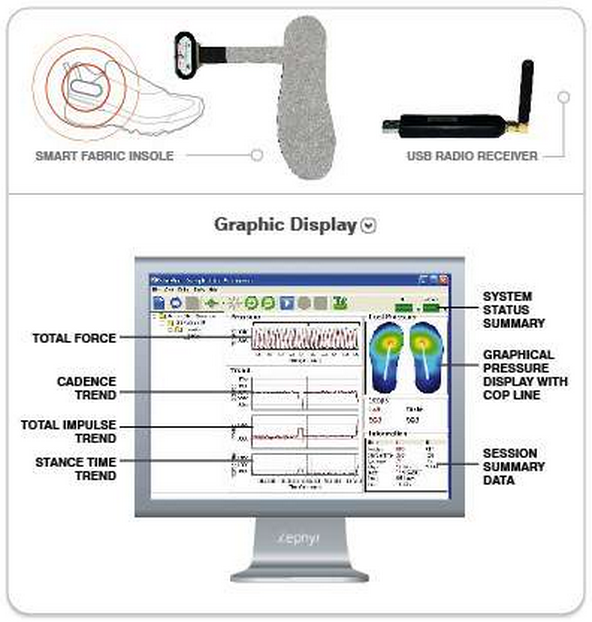
\includegraphics[width=5cm]{billeder/shoepad}
\caption{Figure describing the Shoepad}
\end{wrapfigure}
The system comprises of an insole which has a number of temperature sensors. Theses insoles has a radio transmitter which connects to a computer or watch. The system compares the temperature of both feed and can give an audible or visual alarm if the temperature difference is at a critical level.
\subsubsection{Similarities}
This system will in many ways be very similar to that of the group since the purpose is exactly the same. This system has a number of temperature sensors and the system can based on the values indicate an alarm to the user.
\subsubsection{Differences}
This system is only in the insole and therefore the temperature is only monitored on the bottom of the feet.\\
This system transmits the data via. radio signal and must therefore be within range of the computer which it is connected to. This limits what the user are able to do while wearing the insole.

\subsection{TempTablet}
\textbf{Patent:} none found.
\subsubsection{Description}
\begin{wrapfigure}{r}{5cm}
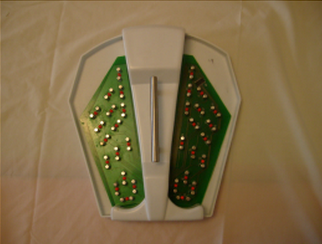
\includegraphics[width=5cm]{billeder/temptablet}
\caption{Image of the TempTablet}
\end{wrapfigure}
The system has a scale/weight-like formfactor and is meant to be used by patients daily. It can store data locally on an SD-card. But it also has some wireless connections although nothing of their use is mentioned in the article.
\subsubsection{Similarities}
The system is meant to be used by patients and monitoring the feet temperature. It can give an alarm depending on the values of these data.
\subsubsection{Differences}
The system is not very mobile because of the formfactor. Therefore it cannot constantly monitor the feet.\\


\subsection{Parotec}
\textbf{Patent:} US5642096
\subsubsection{Description}
Shoe/insole. Hydrocell pressure and temperature sensors. Alarm function.
\subsubsection{Similarities}
The system features a central data unit that collection measurements from the sensors. The data can be transferred to a tool on computer. Based on profiles, the system can warn the user about issues with pressure. 
\subsubsection{Differences}
The sensors are placed in a sole and concentrated around the front of the foot. The system measures pressure. Although mentioned in the patent the system does not measure temperature.
%\begin{table}[H]
%\begin{tabular}{|p{4cm}|p{3.5cm}|p{7cm}|}
%\hline
%Product & Patent & description\\ \hline
%ShoePod Diabetic$^{TM}$ & WO/2009/005373A1 & Shoe/insole. Smart fabric technology. Pressure and temperature sensor arrays. Chip thermistors. \\ \hline
%TempTablet & none & Sensor arrays. Temperature profiles of the feet. Storage of data for comparisons. Alarm function. \\ \hline
%Parotec & US5642096 & Shoe/insole. Hydrocell pressure and temperature sensors. Alarm function. \\ \hline
%\end{tabular}
%\end{table}
%Lignenede devices: \url{http://www.diva-portal.org/smash/get/diva2:359794/FULLTEXT01.pdf} side 17\\

% Evt. aftale om forventet arbejdssted og tid

% Konklusion på det indledende arbejde med forprojektet
\chapter{Konklusion}
We can conclude that the need for this project is real. The prototype will contain the part specified by the project group.\\
A time schedule has been laid out for the project which makes it an achievable goal to have a working prototype based on our specification.\\
We will have to contact health care professions to acquire new knowledge in the field of measuring temperature on feet.\\
There are projects like this already but most of them are not in use or are purely on the experimental state. Although alike there is no project like ours.\\


\end{document}